% Dies ist Teil der Vorlesung Physik auf dem Computer, SS 2012,
% Axel Arnold, Universitaet Stuttgart.
% 
% Dieses Werk ist unter einer Creative Commons-Lizenz vom Typ
% Namensnennung-Weitergabe unter gleichen Bedingungen 3.0 Deutschland
% zugänglich. Um eine Kopie dieser Lizenz einzusehen, konsultieren Sie
% http://creativecommons.org/licenses/by-sa/3.0/de/ oder wenden Sie sich
% schriftlich an Creative Commons, 444 Castro Street, Suite 900, Mountain
% View, California, 94041, USA.
% !TEX root = padc.tex

\chapter{Differentialgleichungen}
\index{Differentialgleichung}

Fast alle physikalischen Vorgänge können durch Differentialgleichungen
(DGLs) beschrieben werden, von der Schrödingergleichung für
Quantensysteme, über die Newtonschen Bewegungsgleichungen bis hin zu
den Navier-Stokes-Gleichungen für Strömungen. Auch das einleitende
Problem des Fadenpendels wurde durch die Differentialgleichung
\begin{equation}
  \ddot\alpha = -\frac{g}{l}\sin(\alpha)
\end{equation}
beschrieben. Die analytische Lösung dieser und der meisten
Differentialgleichungen ist schwierig oder unmöglich, und daher sind
numerische Verfahren zum Lösen von DGLs wichtige Hilfsmittel, um diese
trotzdem untersuchen zu können.

Im Folgenden werden wir numerische Löser für verschiedene Klassen von
Differentialgleichungen kennenlernen. Für gewöhnliche
Differentialgleichungen mit skalarer Variable sind das die
Runge-Kutta-Verfahren, sowie das bereits in der Einleitung
besprochene, sehr gebräuchliche Velocity-Verlet-Verfahren.

Schwieriger ist die Lösung partieller Differentialgleichungen, die
mehrdimensionale Variablen und deren Ableitungen enthalten.  Diese
spielen in der Physik eine besonders wichtige Rolle, weil sie bei
zeit- und ortsabhängigen Prozessen quasi automatisch auftreten. Sie
werden meist mit Hilfe finiter Element-Methoden behandelt, die wir in
dieser Vorlesung aber nur anreissen können. Wir lernen
stattdessen einige Beispiele von partiellen DGLs kennen und wie diese
mit Hilfe finiter Differenzen oder Fouriertransformationen numerisch
gelöst werden können.

\section{Gewöhnliche Differentialgleichungen}
\index{Differentialgleichung>gewöhnliche}
\index{Differentialgleichung>explizite}

Wir betrachten Differentialgleichungen der Form
\begin{equation}
  \label{eq:explicitode}
  y^{(m)}(t) = F(t,\, y(t),\, \dot y(t), \ldots,\, y^{(m-1)}(t))
\end{equation}
mit der gesuchten Lösung $y:\RR\to\RR^n$. Diese heißen gewöhnlich, da
sie nur von einer skalaren Variablen, $t$, abhängen. Wie der Name $t$
schon vermuten lässt, wird diese Variable meist mit der Zeit
assoziiert. Die spezielle Form \eqref{eq:explicitode} wird auch
\emph{explizite} gewöhnliche Differentialgleichung $m$-ter Ordnung
genannt, da wir voraussetzen, dass sich die Gleichung global nach
$y^{(m)}(t)$ auflösen lässt, und $m$ Ableitungen involviert
sind. \emph{Implizite} Gleichungen der Form $F(t, y(t),\,\dot y(t),
\ldots,\,y^{(m)}(t)) = 0$ sind numerisch sehr viel schwieriger zu
lösen, tauchen aber in der Physik auch seltener auf und werden daher
hier nicht weiter besprochen.

Für die numerische Lösung beschränken wir uns weiter auf gewöhnliche
Differentialgleichungen erster Ordnung, also von der Form
\begin{equation}
  \label{eq:1storderode}
  \dot y(t) = F(t,\,y(t)),\quad y(0)\;\text{gegeben}.
\end{equation}
Dies ist keine wirkliche Einschränkung, da sich jede explizite
Differentialgleichung $m$-ter Ordnung in eine höherdimensionale
Gleichung erster Ordnung transformieren lässt:
\begin{equation}
  \frac{d}{dt}\begin{pmatrix}
    y(t)\\
    \dot y(t)\\
    \vdots\\
    y^{(m-1)}(t)
  \end{pmatrix}
  =
  \begin{pmatrix}
    \dot y(t)\\
    \ddot y(t)\\
    \vdots\\
    y^{(m)}(t) = F(t,\, y(t),\, \dot y(t),\, \ldots,\, y^{(m-1)}(t))
  \end{pmatrix}
\end{equation}

Die Differentialgleichung des einleitenden Beispiels
\begin{equation}
  \label{eq:fadenpendel2}
  \ddot \alpha(t) = -\frac{g}{l}\sin \alpha(t),
\end{equation}
wird so zum Beispiel zu
\begin{equation}
  \frac{d}{dt}\begin{pmatrix}
    \alpha(t)\\
    \dot \alpha(t)
  \end{pmatrix}
  =
  \begin{pmatrix}
    \dot \alpha(t)\\
    -\frac{g}{l}\sin \alpha(t),
  \end{pmatrix}.
\end{equation}  
Der Startwert ist genau wie im Eingangskapitel $(\alpha(0),\, \dot
\alpha(0))$, also Anfangsposition und -geschwindigkeit.

\subsection{\keyword{Runge-Kutta-Verfahren}}

Wir suchen eine diskretisierte Näherung $y_n \approx y(t_n)$
für das Problem~\eqref{eq:1storderode} mit
äquidistanten Zeitpunkten $t_n=n h$, $n=0,\,1,\,\ldots$, also Schrittweite
$h$. Es gilt
\begin{equation}
  y(t_{n+1}) = y(t_n+h) = y(t_n) + \int_{t_n}^{t_n+h} \dot y(t)\,dt
  =  y(t_n) + \int_{t_n}^{t_n+h} F[t,\, y(t)]\,dt.
\end{equation}
Da $y_0 = y(0)$ gegeben ist, liegt es nahe, $y_1 \approx y(h)$ durch
numerische Integration zu bestimmen, dann $y_2 \approx y(2h)$ durch
numerische Integration aus $y_1$ und so weiter. Das Problem dabei ist,
dass der Integrand $F[t,\, y(t)]$ die zu findende Funktion $y$
enthält. Um also $y(t)$ an Stellen $t\in [t_n,\, t_n + h]$ annähern zu
können, müssen wir einige Werte von $y$ in diesem Intervall wiederum
durch Integration gewinnen. Dies führt zur allgemeinen Form eines
$s$-stufigen Runge-Kutta-Verfahrens
\begin{equation}
  y_{n+1} = y_n + h\sum_{j=1}^s b_j k_j
\end{equation}
mit den Näherungen für $F[t_n + hc_j,\, y(t_n + h c_j)]$
\begin{equation}
  \label{eq:rkkj}
  k_j = F\left(t_n + h c_j,\, y_n + h \sum_{k=1}^s a_{jk} k_k\right).
\end{equation}
$b,\,c\in\RR^s$ und $A=(a_{jk})\in\RR^{s,s}$ sind dabei Konstanten,
die das Verfahren beschreiben. $c$ gibt die Zeitpunkte an, an denen
$F[t,\,y(t)]$ im Intervall $[t,\,t+h]$ angenähert wird, in Vielfachen
der Schrittweite $h$. $c_i=0$ besagt also, dass $k_i\approx
F[t_n,\,y(t_n)]$, $c_i=1$, dass $k_i\approx F[t_n + h,\,y(t_n + h)]$.
$A$ gibt die Quadraturgewichte für die Zwischennäherungen an, $b$ die
Quadraturgewichte der Endnäherung. Diese Konstanten sind dabei nicht
nur von $F$ unabhängig, sondern auch von der Schrittweite $h$, so dass
ein Runge-Kutta-Schema durch Verkleinern der Schrittweite im Prinzip
beliebig genau gemacht werden kann.  Die Zwischenwerte $k_j$
erscheinen auf beiden Seiten von~\eqref{eq:rkkj}, es handelt sich also
um ein gekoppeltes, implizites Gleichungssystem.  Ist
$F(t,\,y)$ eine nichtlineare Funktion, ist eine solche Gleichung nur
aufwändig zu lösen.

\index{Runge-Kutta-Verfahren>explizite}%
Daher werden meist \emph{explizite} Runge-Kutta-Verfahren verwendet,
bei denen $A$ eine linke untere Dreiecksmatrix mit Nulldiagonale ist,
also $a_{jk} = 0$ für $k\ge j$. Dann werden zur Berechnung von $k_j$
nur $k_k$, $k=1(1)j-1$ benötigt, die bereits berechnet sind. Eine
Implementierung eines Runge-Kutta-Verfahrens ähnelt dann sehr dem
Gauß-Seidel-Verfahren, das ebenfalls die Zeilen der zu lösenden
Matrix sequentiell abarbeitet.

Dass man trotzdem auch implizite Verfahren, also mit allgemeiner
Matrix, in Betracht zieht, hängt damit zusammen, dass diese stabiler
sind, und auch sogenannte steife DGLs lösen können. Ist $A$ linke
untere Dreiecksmatrix, aber die Diagonale nicht Null, spricht man von
DIRKs, diagonal-impliziten Runge-Kutta-Verfahren. Diese lassen sich
noch mit verhältnismäßig begrenztem Aufwand lösen, da pro $k_j$
lediglich eine eindimensionale Gleichung gelöst werden muss.

Der Fehler von Runge-Kutta-Verfahren wird üblicherweise durch die
Konvergenz- und Konsistenzordnung beschrieben. Die Konvergenzordnung
$p$ besagt, dass die Näherung gleichmäßig gegen $f(t_n)$ konvergiert, also
$\max \norm{y_n - y(t_n)} = \O(h^p)$. Die Konvergenz ist
meist schwer zu beweisen, einfacher ist die Konsistenzordnung $p$, die
nur fordert, dass $\norm{y_{n+1} - y(t_{n+1})} = \O(h^p)$, falls
$y_n=y(t_n)$. Konsistenz besagt also lediglich, dass ein Schritt
prinzipiell konvergiert. Ist die Funktion $F$ Lipschitz-stetig, also
etwa genügend glatt, dann gilt allerdings Konsistenzordnung =
Konvergenzordnung.

\index{Butcher-Tableau}%
Im Folgenden werden einige der gebräuchlicheren Runge-Kutta-Verfahren
angegeben. Dabei hat sich das \emph{Butcher-Tableau}
\begin{center}
  \renewcommand{\arraystretch}{1.3}
  \begin{tabular}{r|l}
    c & A \\\hline
    & $b^T$
  \end{tabular}
\end{center}
als kurze Darstellung etabliert. Die $j$-te Zeile gibt dabei an, zu
welchen Zeitpunkt $t_n + hc_j$ die Näherung $k_j$ berechnet wird und
welchen Quadraturgewichte benutzt werden. $b_j$ sind die
Quadraturgewichte der für die finale Integration zu $y_{n+1}$.

Die Konstanten ergeben sich im Prinzip aus den benutzten
Quadraturformeln. Allerdings gibt es neben der Bedingung, dass die
Formeln möglichst explizit sein sollten, noch weitere
Stabilitätsbedingungen, die hier aber nicht beschrieben werden
können. Daher kann man nicht einfach beliebige Quadraturformeln
kombinieren, sondern sollte bei den im Folgenden beschriebenen,
gebräuchlichen Formeln bleiben.

\subsubsection{Explizites Eulerverfahren}
\index{Eulerverfahren>explizites}

\begin{center}
  \renewcommand{\arraystretch}{1.3}
  \begin{tabular}{r|l}
    0 & \\\hline
    & 1
  \end{tabular}
\end{center}
Dieses Butcher-Tableau besagt nichts anderes, als dass
\begin{equation}
  y_{n+1} = y_n + h F(t_n,\, y_n) \approx y(t_n) + h \dot y(t_n).
\end{equation}
Es handelt sich also um die direkte Integration per Rechteckregel, und
damit um ein Verfahren der Ordnung 1, \dh mit globalem Fehler
$\O(h)$. Dieses Verfahren entspricht der einfachen
Integration~\eqref{eq:simple} im einleitenden Beispiel. Das explizite
Eulerverfahren ist nicht sehr genau und nur für global
Lipschitz-stetige $F$ stabil. Daher sollte man es bei praktischen
Anwendungen im Allgemeinen vermeiden.

\subsubsection{Implizites Eulerverfahren}
\index{Eulerverfahren>implizites}

\begin{center}
  \renewcommand{\arraystretch}{1.3}
  \begin{tabular}{r|l}
    1 & 1\\\hline
    & 1
  \end{tabular}
\end{center}
Wie der Name schon sagt, ist dies ein implizites Verfahren, genauer,
ein DIRK, bei dem in jedem Schritt die Gleichung
\begin{equation}
  k_1 = F(t_{n+1},\,y_n + h k_1)
\end{equation}
gelöst werden muss, um die neue Näherung $y_{n+1} = y_n + h k_1$ zu
berechnen. Durch Einsetzen ergibt sich
\begin{equation}
  y_{n+1} = y_n + h F(t_{n+1},\, y_{n+1}),
\end{equation}
das implizite Eulerverfahren ist also ebenfalls eine Rechteckregel,
aber mit dem neu zu bestimmenden Punkt $y_{n+1}$ als Aufpunkt. Die
Ordnung dieses Verfahrens ist daher ebenfalls 1. Anders als das
explizite Eulerverfahren ist das implizite Eulerverfahren allerdings
ziemlich stabil, auch wenn $F$ nicht Lipschitz-stetig ist. Der
Nachteil ist, dass in jedem Schritt eine nichtlineare Gleichung gelöst
werden muss, was das Verfahren recht aufwändig macht.

\subsubsection{Das Runge-Kutta-Verfahren}
\index{Runge-Kutta-Verfahren>4. Ordnung}

\begin{center}
  \renewcommand{\arraystretch}{1.3}
  \begin{tabular}{r|llll}
    0 & \\
    $\nicefrac{1}{2}$ & $\nicefrac{1}{2}$ \\
    $\nicefrac{1}{2}$ & 0 & $\nicefrac{1}{2}$ \\
    1 & 0 & 0 & 1 \\
    \hline
    & $\nicefrac{1}{6}$ &  $\nicefrac{1}{3}$ & 
    $\nicefrac{1}{3}$ &  $\nicefrac{1}{6}$
  \end{tabular}
\end{center}
Dies ist das klassische Runge-Kutta-Verfahren, das zuerst 1901 von
Kutta beschrieben wurde. Wird in der Literatur von "`dem
Runge-Kutta-Verfahren"' ohne weitere Angaben gesprochen, ist daher
dieses Verfahren gemeint. Bei genügend glattem $f$ hat es
Konvergenzordnung 4, ist also deutlich besser als die Eulerverfahren.

Wie können wir das Tableau verstehen?  Wir setzen
$\tau=\nicefrac{h}{2}$. Die zweite und dritte Zeile bestimmen zwei
Näherungen für $F[t_n+\tau, y(t_n+\tau)]$, zunächst mit Hilfe der
linken ($k_2$), und dann der rechten Ableitung ($k_3$). $k_4$ ist dann
eine Näherung für $F[t_n+h, y(t_n+h)]$. Diese Näherungen werden in die
Simpsonregel eingebracht, wobei $k_2$ und $k_3$ mit gleichen Gewichten
eingehen.

\subsubsection{Beispielimplementation}

Eine Python-Implementation des allgemeinen Runge-Kutta-Schemas für
$\dot y(t) = $\argd{F}$[t, y(t)]$, $y(0) =$ \argd{y0} könnte wie folgt
aussehen:%
\lstinputlisting[firstline=10,lastline=34]{rk.py}%
Die Lösung $y(t)$ kann dabei auch vektorwertig sein, dann müssen
\argd{y0} und der Rückgabewert der Funktion \argd{F} gleich große
NumPy-Arrays sein. Die Integration findet stets von $t=0$ bis
\argd{tmax} statt, in Schritten der Weite \argd{h}.  Die Routine
liefert das Ergebnis als Matrix aus den Zeit- und Lösungspunkten
zurück. Die erste Spalte enthält den Zeitpunkt $t_n$, die zweite die
erste Komponente von $y_n$, die dritte die zweite Komponente \usw

Die Funktion \lstinline!rk_explicit! kann beliebige, explizite
Runge-Kutta-Verfahren durchführen.  Dazu erwartet sie als ersten
Parameter ein Wörterbuch, dass das Butchertableau für das zu
benutzende Runge-Kutta-Verfahren beschreibt. Für das Eulerverfahren
und das klassische Runge-Kutta-Verfahren sehen solche Wörterbücher so
aus:%
{\lstinputlisting[firstline=36]{rk.py}}%

\subsection{Beispiel: Lotka-Volterra-Gleichungen}
\index{Lotka-Volterra-Gleichungen}

\begin{figure}
  \centering
  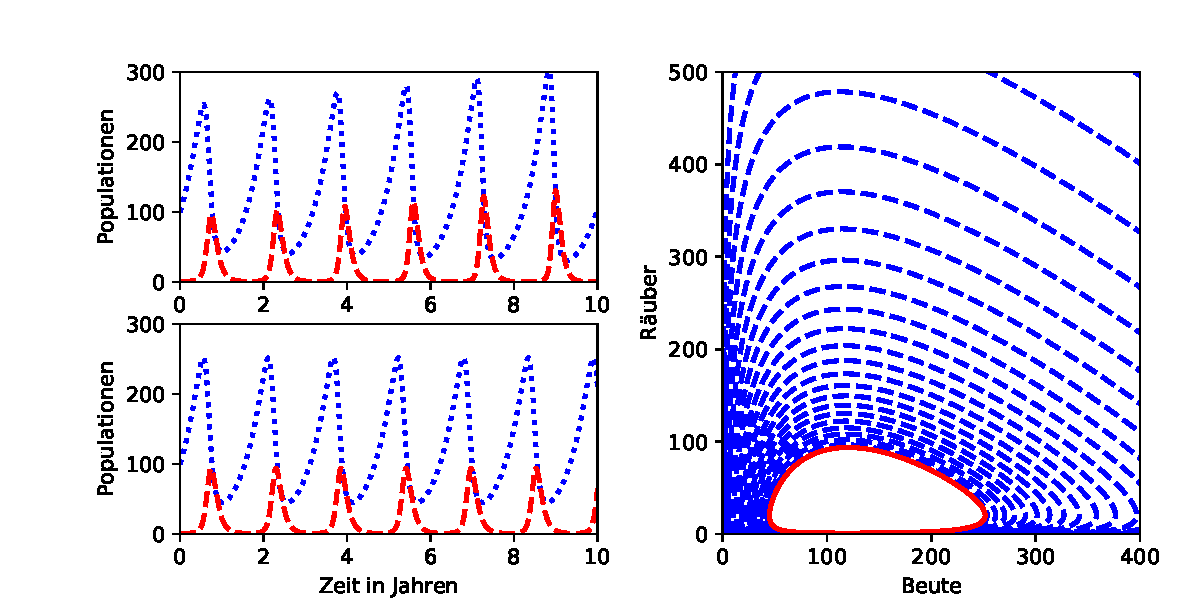
\includegraphics[width=\textwidth]{plots/lotka-volterra}
  \caption{Lösungen der Lotka-Volterra-Gleichungen mit dem einfachen
    Eulerverfahren (oben links) und dem Runge-Kutta-Verfahren (unten
    links). Blau gepunktet ist die Beutepopulation, rot gestrichelt
    die Räuberpopulation. Rechts das Räuber-Beute-Diagramm für das
    Eulerverfahren (blau gestrichelt) und das Runge-Kutta-Verfahren
    (rot durchgezogen). Während das Verfahren vierter Ordnung die
    erwartete periodische Trajektorie ergibt, wächst mit dem
    Eulerverfahren die Spitzenpopulation immer weiter. Dies zeigt die
    Instabilität des Eulerverfahrens.}
  \label{fig:lotka}
\end{figure}

Die Lotka-Volterra-Gleichungen sind nach A.~J.~Lotka und V.~Volterra
benannt, die diese 1925 als einfaches Modell für die
Populationsdynamik eines Räuber-Beute-Systems angegeben hatten, also,
wie sich die Populationsgrößen von Räubern und Beute im zeitlichen
Verlauf ändern. Die Gleichungen beruhen auf stark vereinfachenden
Annahmen, nämlich, dass den Beutetieren unbegrenzte Resourcen zur
Verfügung stehen, während die Räuber ausschließlich auf die Beutetiere
angewiesen sind. Trotzdem lassen sich die qualitativen Vorhersagen
dieses Modells in der Natur verifizieren, an so unterschiedlichen
Systemen wie zum Beispiel Haie und Fische oder Wölfe und Hasen.  Es
gibt Erweiterungen mit begrenzten Resourcen, oder mehrstufigen
Systemen (also etwa Haie, Fische und Plankton), die aber nicht
wesentlich mehr zum Verständnis beitragen.

Die klassischen Lotka-Volterra-Gleichungen sind zwei gekoppelte
Differentialgleichungen für die Populationen $N_R$ der Räuber und
$N_B$ der Beutetiere:
\begin{equation}
  \label{eq:lotka-volterra}
  \frac{d}{dt}
  \begin{pmatrix}
    N_B\\
    N_R
  \end{pmatrix}
  = F(N_B, N_R) = 
  \begin{pmatrix}
    A N_B  - B N_BN_R\\
    -C N_R + D N_BN_R
  \end{pmatrix}.
\end{equation}
Dabei gibt $A$ die Vermehrungsrate der Beutetiere an, die nur von der
aktuellen Populationsgröße abhängt und $B$ die Rate, mit der ein
Räuber ein Beutetier auffrisst. $C$ gibt die Sterberate der Räuber an,
und $D$ die Rate, mit der sich ein Räuber vermehrt, wenn er ein
Beutetier gefangen hat. Die Räuber müssen also Beutetiere fangen, um
sich zu vermehren, während die Beutetiere sich von selber
vermehren. Sind also keine Räuber vorhanden, vermehren sich die
Beutetiere exponentiell, sind keine Beutetiere vorhanden, sterben die
Jäger exponentiell aus.

Im Folgenden betrachten wir ein solches System aus Hasen und
Wölfen. Es sei $A=2$ Hasen pro Jahr, \dh ein Hasenpaar hat vier
Nachkommen im Jahr, und $B=0,1$, ein Wolf fängt also im Schnitt alle
10 Jahre einen bestimmten Hasen. Die tatsächliche Fangrate hängt
natürlich von der Menge der Wölfe und Hasen ab. Gibt es viele Hasen
oder Wölfe, ist die Chance, dass irgendein Wolf irgendeinen Hasen
fängt, gut. Die Wölfe hingegen sind recht hungrig, wir setzen daher
$C=12$. Ein Wolf stirbt also in etwa einem Monat, wenn er keinen Hasen
fängt. Umgekehrt reicht ein Hase kaum, um sich zu vermehren, daher
setzen wir $D=0,1$, so dass etwa 10 Hasen zur erfolgreichen Vermehrung
gefressen werden müssen.

Nachdem wir nun die Raten festgelegt haben, können wir zum Beispiel
ein Runge-Kutta-Verfahren benutzen, um \eqref{eq:lotka-volterra} zu
lösen. Dazu müssen wir noch einen Startwert festlegen, hier hundert
Hasen und einen Wolf, und eine Schrittweite, die wir auf einen Tag,
also $1/365$-tel, setzen. Abbildung~\ref{fig:lotka} zeigt die
resultierenden Populationen, einmal als Funktion der Zeit und einmal
als Räuber-Beute-Diagramm.

Charakteristisch für die Lotka-Volterra-Gleichungen ist ein
periodisches Verhalten, wie man analytisch zeigen kann. Dabei gibt es
lediglich zwei Gleichgewichtszustände, den man leicht bestimmen kann:
\begin{equation}
  0 \stackrel{!}{=}
  \begin{pmatrix}
    N_B (A - B N_R)\\
    N_R (-C + D N_B)
  \end{pmatrix}
  \implies N_B=N_R=0\;
  \text{oder}\;N_B=\frac{C}{D}\;\text{und}\;N_R=\frac{A}{B}.
\end{equation}
In unserem Fall wären die Populationen also bei $N_B=120$ und $N_R=20$
stabil. Unser davon leicht abweichender Startwert sollte zu einer
Trajektorie führen, die um diesen Fixpunkt periodisch kreist. Dies ist
auch tatsächlich der Fall, wenn das Runge-Kutta-Verfahren, das vierte
Ordnung hat, benutzt wird. Dabei ist gut zu beobachten, dass die
Wolfspopulation der Hasenpopulation folgt. Zunächst wächst die
Hasenpopulation nahezu ungebremst exponentiell, bis die
Wolfspopulation nachzieht. Daraufhin dezimieren die Wölfe die
Hasenpopulation rasch und sterben in der Folge selber nahezu
aus. Dadurch nimmt die Hasenpopulation wieder exponentiell zu, und der
Zyklus beginnt von neuem. Das Nachlaufen der Räuberpopulation ist
charakteristisch für die Lotka-Volterra-Gleichungen und kann auch in
der Natur beobachtet werden.

Wird zur Integration statt des Runge-Kutta-Verfahrens das
Eulerverfahren benutzt, nehmen beide Populationen mit der Zeit immer
weiter zu. Wie vorher gesagt, sind die Lösungen der
Lotka-Volterra-Gleichungen aber periodisch, sofern es Räuber gibt. Die
Zunahme ist also nur ein numerisches Artefakt. Selbst wenn der
Zeitschritt um einen Faktor 10 gesenkt wird, driften die mit dem
Eulerverfahren berechneten Populationen während der gezeigten 10 Jahre
um etwa 10 Individuen. Dies zeigt eindrücklich die Instabilität des
Eulerverfahrens.

\subsection{Velocity-Verlet-Verfahren}
\index{Velocity-Verlet-Verfahren}

In der Einleitung hatten wir bereits besprochen, dass die
Fadenpendelgleichung~\eqref{eq:fadenpendel2} mit Hilfe des
Velocity-Verlet-Verfahrens numerisch gelöst werden kann. Dieses dient
zur Lösung von Differentialgleichungen der Form
\begin{equation}
  \ddot x(t) = F[t,\, x(t)],
\end{equation}
also gewöhnlichen Differentialgleichungen zweiter Ordnung, die nicht
von der Geschwindigkeit $\dot x(t) = v(t)$ abhängen. Diese Form ist
typisch für Bewegungsgleichungen mit konservativen Kräften, daher ist
das Velocity-Verlet-Verfahren zum Beispiel das Standard-Verfahren für
die Propagation von klassischen Vielteilchensystemen und spielt eine
wichtige Rolle in gängigen Programmen zur Molekulardynamik. Diese
integrieren mit Hilfe eben dieses Verfahrens die Bewegungsgleichungen
für unter Umständen mehrere Milliarden Atome!

Auch bei dieser Methode wird die Lösung $x_n\approx x(t_n)$
äquidistant mit Schrittweite $h$ diskretisiert und wie folgt
berechnet:
\begin{align}
  v_{n+\nicefrac{1}{2}} &= v_n + \frac{h}{2} F(t_n, x_n) \nonumber\\
  x_{n+1} &= x_n + h v_{n+\nicefrac{1}{2}} \\
  v_{n+1} &= v_{n+\nicefrac{1}{2}} + \frac{h}{2} F(t_{n+1}, x_{n+1}).\nonumber
\end{align}
Ähnlich wie bei den Runge-Kutta-Verfahren wird also ein
Zwischenschritt bei $h/2$ eingelegt, allerdings nur für die Berechnung
von $v_{n+\nicefrac{1}{2}}\approx x'(t_n + \nicefrac{h}{2})$.  Dabei
wird dieselbe Beschleunigung $F(t_n, x_n)$ in aufeinanderfolgenden
Zeitschritten zweimal benötigt. In Molekulardynamiksimulationen mit
vielen Atomen ist die Berechnung der Kräfte meist recht teuer, daher
speichert man die Kräfte üblicherweise zwischen.

Um die Ordnung dieses Verfahrens zu bestimmen, eliminieren wir die
Geschwindigkeiten:
\begin{align}
  x_{n+1} &= x_n + h v_n + \frac{h^2}{2} F(t_n, x_n)\nonumber\\
  &=  x_n + h v_{n-\nicefrac{1}{2}} + h^2F(t_n, x_n)\nonumber\\
  &=  x_n + x_n - x_{n-1} + h^2F(t_n, x_n)
  =  2 x_n - x_{n-1} + h^2F(t_n, x_n)
\end{align}
Die ist eine finite Differenz gemäß \eqref{eq:1order2diff}, für die
\begin{equation}
  \frac{x_{n+1}  - 2 x_n + x_{n-1}}{h^2} = F(t_n, x_n) + \O(h^2)
\end{equation}
gilt. Der Fehler in $x_{n+1}$ ist also von der Größenordnung
$\O(h^4)$, sofern $x_n$ und $x_{n-1}$ oder $v_n$ exakt waren. Die
Geschwindigkeiten haben offenbar einen Fehler der Ordnung $\O(h^2)$.

Das Velocity-Verlet-Verfahren ist von der Implementation her
vergleichbar einfach wie das Eulerverfahren, aber anders als dieses
recht stabil und hat, wie gezeigt, eine sehr gute Konsistenzordnung,
vergleichbar mit dem Runge-Kutta-Verfahren. Es hat aber noch eine
andere wichtige Eigenschaft: anders als die Runge-Kutta-Verfahren ist
das Verfahren \emph{symplektisch}, was bedeutet, dass es keine
Energiedrift zulässt, und zum anderen besonders gut geeignet ist, in
Molekulardynamiksimulationen Observablen über den Phasenraum zu
mitteln.  Auch das Simulationspaket ESPResSo, mit dem zum Beispiel im
vorigen Kapitel die Simulationen zum Simulated Annealing durchgeführt
wurden, oder das in der Biophysik populäre NAMD~\cite{namd} benutzen
daher einen Velocity-Verlet-Integrator.

\subsubsection{Beispielimplementation}

Eine Python-Implementation des Velocity-Verlet-Verfahrens für $\ddot
x(t) = $\argd{F}$[t, x(t)]$ mit $x(0) =$ \argd{x0} und $v(0) =$
\argd{v0} könnte wie folgt aussehen:%
\lstinputlisting[firstline=10]{vv.py}%
Genau wie beim Runge-Kutta-Beispiel kann die Lösung $x(t)$ auch
vektorwertig sein, wenn \argd{x0}, \argd{v0} und der Rückgabewert der
Beschleunigungsfunktion \argd{F} gleichgroße NumPy-Arrays
sind. Integriert wird von $t=0$ bis \argd{tmax} in Schritten der Weite
\argd{h}. Die Routine liefert das Ergebnis als Matrix aus den Zeit-
und Lösungspunkten sowie den Geschwindigkeiten zurück. Ein Eintrag hat
also die Form $\left(t^{(k)}, x^{(k)}_1,\ldots,x^{(k)}_n,
v^{(k)}_1,\ldots,v^{(k)}_n\right)$.

Die obige Implementation ist nicht sehr effizient, da die
Kraftfunktion in zwei aufeinanderfolgenden Zeitschritten zweimal an
der selben Stelle ausgewertet wird, statt die Werte
zwischenzuspeichern.

\subsection{Beispiel: 3-Körperproblem}
\index{Mehrkörperproblem}

\begin{figure}
  \centering
  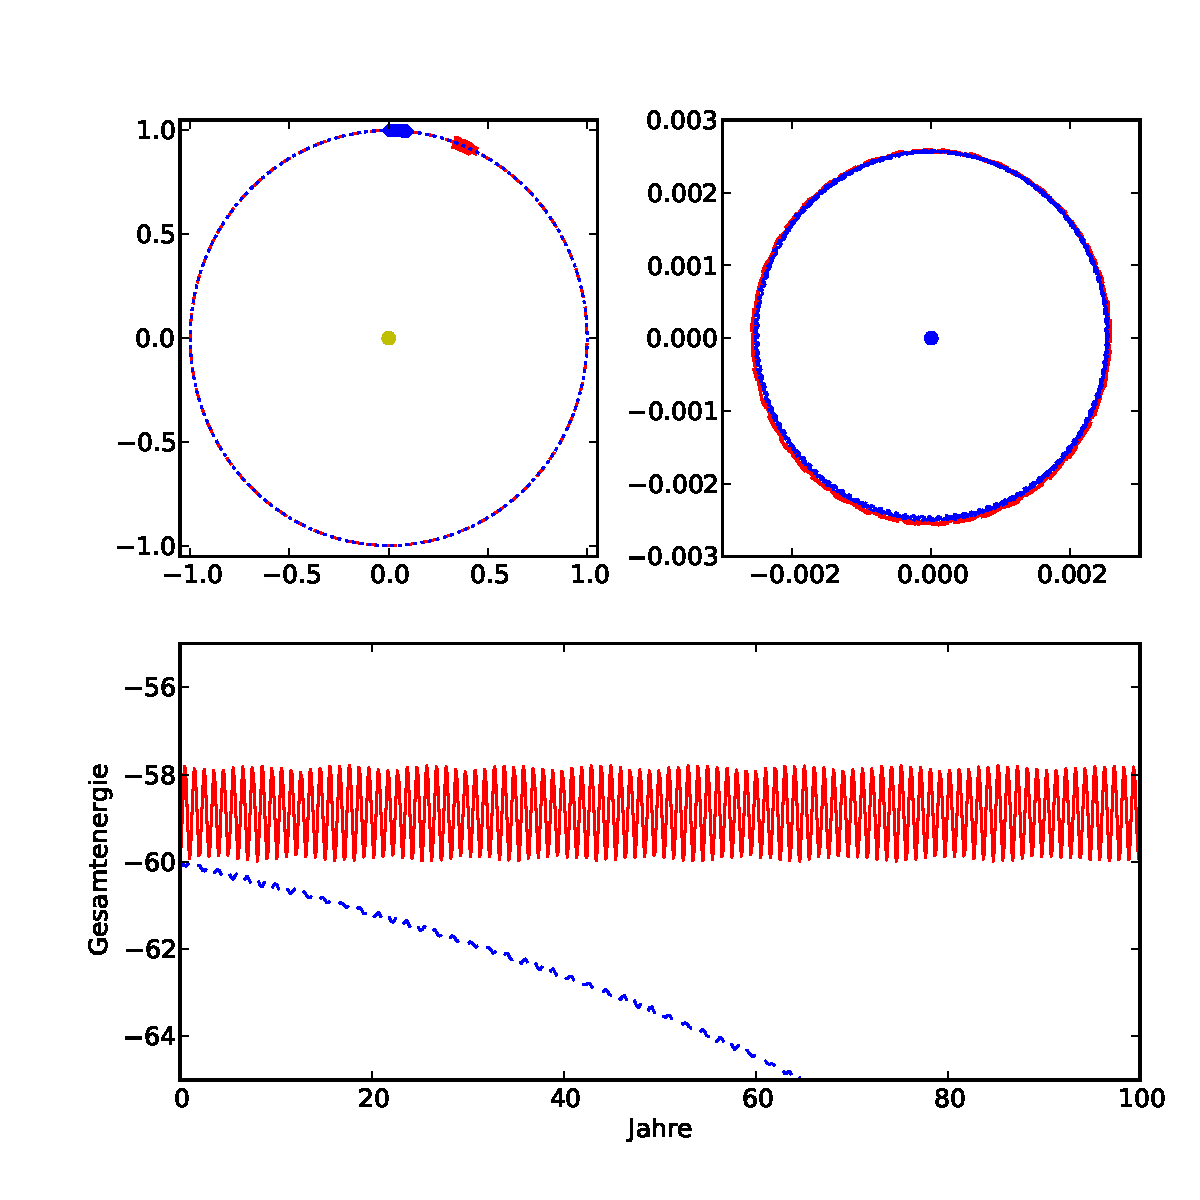
\includegraphics[width=\textwidth]{plots/planets}
  \caption{Oben: Simulierte Bahn der Erde um die Sonne während 10
    Jahren (links) und des Monds um die Erde während eines halben
    Jahres (rechts). Rot gestrichelt sind die vom
    Velocity-Verlet-Verfahren berechneten Bahnen, blau gepunktet die
    des Runge-Kutta-Verfahrens. Rote Sterne bzw.\ blaue Rauten auf den
    Erdbahnen bezeichnen Punkte im Abstand von 365 Tagen, also etwa
    einem Jahr. Aufgrund der kleinen Abstände sind die Schwankungen in
    der Mondbahn größer, aber bei beiden Verfahren akzeptabel. Unten:
    Energien bei einer Rechnung mit größerer Simulationslänge und
    Zeitschritt. Hier zeigt sich die Symplektizität des
    Velocity-Verlet-Verfahrens, das die Energie im Mittel erhält,
    während das Runge-Kutta-Verfahren driftet.}
  \label{fig:planets}
\end{figure}

Wir betrachten die klassischen Bahnen von Sonne, Erde und Mond unter
Vernachlässigung anderer Himmelskörper und der nicht ganz korrekten
Annahme, dass alle drei Körper in einer Ebene kreisen. Dieses System
hat den Vorteil, dass die Kreisbahn des Mondes um die Erde sehr klein
gegenüber der Kreisbahn des Erde-Mond-Systems um die Sonne ist, so
dass das Problem sehr unterschiedliche Längenskalen aufweist, die der
Integrator stabil integrieren muss.

Zwischen den Objekten mit Positionen $r_i$ und Massen $m_i$ wirkt die
nichtrelativistische Gravitationskraft
\begin{equation}
  F_{ij} = -\frac{G m_1 m_2}{\norm{r_i - r_j}^3}\left(r_i - r_j\right)
\end{equation}
mit der Gravitationskonstanten $G$. Die gesamte Kraft auf ein Objekt
berechnet sich als
\begin{equation}
  F_{i} = \sum_{j\neq i} F_{ij}.
\end{equation}
Letztere Gleichung gilt natürlich für ein beliebiges
Mehrkörperproblem, nur die Paarwechselwirkungen $F_{ij}$ ändern sich
je nach den wirkenden Kräften. Auf molekularer Ebene ist die
Gravitation vernachlässigbar, dafür wirken zum Beispiel
elektrostatische und van der Waals-Kräfte.

Wie eingangs besprochen, ist es sinnvoll, die Einheiten so zu wählen,
dass die relevanten Variablen in der Größenordnung von eins liegen, so
dass man von einem Implementationsfehler ausgehen kann, wenn plötzlich
sehr große Werte auftreten. In diesem Fall wählen wir als
Längeneinheit die astronomische Einheit, die dem mittleren Abstand
zwischen Sonne und Erde entspricht, und messen Zeiten in Jahren, was
in etwa der Umdrehungszeit der Erde um die Sonne entspricht. Massen
messen wir entsprechend in Erdenmassen $m_E$. In diesem System ist zum
Beispiel $G=1,1858\cdot 10^{-4} AU^3 m_E^{-1} a^{-2}$. Die Sonne hat
$333.000$ Erdenmassen, der Mond wiegt hingegen nur $0,0123m_E$ und
befindet sich etwa $0,00257AU$ von der Erde entfernt. Das verdeutlicht
nochmals die unterschiedlichen Skalen, mit denen der Integrator
zurechtkommen muss.

Abbildung~\ref{fig:planets} oben zeigt die resultierenden Bahnen der
Erde um die Sonne und des Monds um die Erde für die Dauer von 10
Jahren. Die Schrittweite beträgt ein $\nicefrac{1}{365}$-tel Jahr,
also etwa einem Tag, integriert wird mit dem Velocity-Verlet-Verfahren
und dem Runge-Kutta-Verfahren, die beide vierter Ordnung sind. Beide
Verfahren reproduzieren die Erd- und auch Mondbahnen recht gut, auch
wenn die Mondbahn aufgrund der kleinen Abstände stärkere Schwankungen
zeigt. Auf der Erdbahn wurden Punkte im Abstand eines Jahres markiert,
die, wie man erwarten würde, dicht beieinander liegen. Für die
Qualität dieser Kurzzeitbahnen ist der Velocity-Verlet also mit dem
Runge-Kutta-Verfahren der gleichen Ordnung vergleichbar.

Im unteren Teil ist gezeigt, wie sich die beiden Verfahren verhalten,
wenn nicht nur deutlich länger, sondern auch mit größeren Zeitschritt
simuliert wird. Für einen Zeitschritt von 20 Tagen und einer Länge
von 100 Jahren ist der Velocity-Verlet-Integrator
überlegen, denn er zeigt zwar größere Energieschwankungen, erhält aber
langfristig die mittlere Energie. Das Runge-Kutta-Verfahren hingegen
zeigt eine deutliche Energiedrift, die das System langfristig
kollabieren lässt.

Man sollte allerdings beachten, dass für beide Integratoren die
Mondbahnen vollkommen falsch sind, der Mond verlässt sogar seine
Erdumlaufbahn! Für astrophysische Simulationen ist so etwas natürlich
nicht akzeptabel, aber in der Molekulardynamik spielen die exakten
Trajektorien der Moleküle keine Rolle, da sie sowieso nicht gemessen
werden können. Zudem sind molekulare Systeme hochchaotisch, \dh
selbst bei winzigen Störungen weichen Trajektorien nach kurzer Zeit
stark ab. In diesem Fall ist die Energieerhaltung des
Velocity-Verlet-Algorithmus sehr wichtig, denn sie garantiert, dass
trotzdem das korrekte statistische Ensemble simuliert wird und die
Messungen sinnvoll sind, selbst wenn die Trajektoren selber nur auf
sehr kurzen Zeitabschnitten sinnvoll sind.

\section{Partielle Differentialgleichungen}
\index{Differentialgleichung>partielle}

Die numerische Lösung von partiellen Differentialgleichungen, also
Differentialgleichungen in mehreren Variablen, ist erheblich
komplexer. Meist werden diese Art von Differentialgleichungen über
Finite-Elemente-Methoden (FEM) gelöst, andere Methoden sind
Finite-Volumen-Methoden (FVM) oder die Finite-Differenzen-Methode
(FDM). In einigen Fällen können Differentialgleichungen auch durch
schnelle Fouriertransformation numerisch gelöst werden.

Das Ziel bei diesen Ansätzen ist immer gleich: die Differentialgleichung
soll in eine algebraische Gleichung überführt werden, für die wir ja bereits effiziente Lösungsmethoden kennen.

\subsection{Finite-Differenzen-Methode --- Wärmeleitungsgleichung}
\index{Diffusionsgleichung}
\index{Wärmeleitungsgleichung}
\index{Schrödingergleichung}
\index{Finite-Differenzen-Methode}
\index{FDM}
\index{Lösung partieller DGLs>FDM}

\begin{figure}
  \centering
  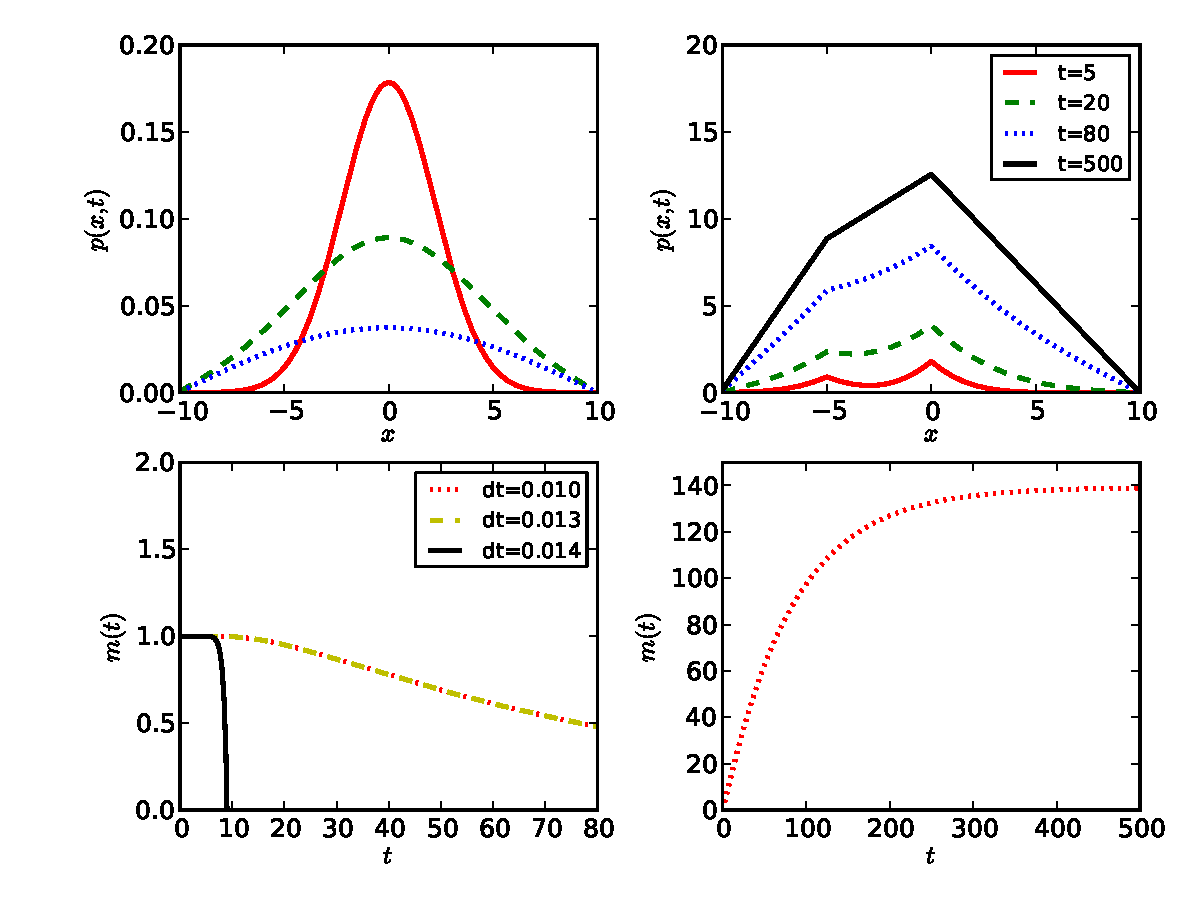
\includegraphics[width=\textwidth]{plots/waermeleitung}
  \caption{Näherungen für die Diffusionsgleichung. Oben die Lösungen
    zu unterschiedlichen Zeitpunkten $t$ für eine $\delta$-verteilte
    Anfangsverteilung (links) und zwei Quellen konstanter Rate 1 bei 0
    und $\nicefrac{1}{2}$ bei -5 (rechts). Unten sind die
    korrespondieren Gesamtmassen angegeben. Für die
    $\delta$-Verteilung sind die Gesamtmassen auch bei geringfügig
    höheren Zeitschritten $\delta t$ angegeben, wobei für $\delta
    t=0,014$ die Näherung versagt.}
  \label{fig:waermeleitung}
\end{figure}

Ist das interessante Gebiet $\Omega$ hinreichend einfach, reichen
die einfachen finite Differenzen, wie wir sie bereits kennengelernt haben, um partielle
Differentialgleichungen zu diskretisieren.  Wir betrachten als
Beispiel die Differentialgleichung
\begin{equation}
  \label{eq:diffdgl}
  \frac{\delta}{\delta t} p(x, t) =
  D\frac{\delta^2}{\delta x^2} p(x, t).
\end{equation}
Gesucht ist $p:\RR^n\times\RR\to\RR$, $D$ ist ein freier Parameter,
die Diffusionskonstante. Diese Differentialgleichung hatten wir in
Abschnitt~\ref{sec:rw} als Diffusionsgleichung kennengelernt. Meist
wird diese Gleichung aber als Wärmeleitungsgleichung bezeichnet, weil
sie auch die Wärmeleitung beschreibt. Auch die zeitabhängige
Schrödingergleichung hat diese Form, ist allerdings komplexwertig.

Um die Differentialgleichung zu lösen, diskretisieren wir wie gewohnt
die Raumkoordinaten äquidistant mit Abstand $h$, d.\,h.\, wir setzen
$x_k = kh$ und $p_k(t) = p(x_k, t)$ für $k=1(1)N$. Für die zweite
Ableitung kennen wir bereits eine einfache Strategie: wir ersetzen sie
durch eine finite Differenz auf dem Gitter, etwa
\eqref{eq:1order2diff}. Das ergibt in einer Dimension die
ortsdiskretisierte Differentialgleichung
\begin{equation}
  \label{eq:discrdiff}
  \frac{\delta}{\delta t} p_k(t) =
  \frac{D}{h^2} \left[p_{k-1}(t) - 2 p_k(t) + p_{k+1}(t)\right].
\end{equation}
Aus der partiellen Differentialgleichung ist eine gewöhnliche
Differentialgleichung in $t$ mit $N$ Variablen
$p_1(t),\ldots,p_N(t)$ geworden, wobei $N$ die Anzahl der Ortspunkte
ist. Diese DGL lösen wir nun mit dem Runge-Kutta-Verfahren. Das hat
den großen Vorteil, dass wir die Verteilungen $p_k(t) = p(x_k, t)$, die bei
großem $N$ oder mehreren Dimensionen sehr groß werden können, nur für
wenige Zeitschritte speichern müssen.

Quellcode~\ref{lst:waermeleitung} zeigt den resultierenden Code, der
die Runge-Kutta-Implementierung aus diesem Kapitel nutzt. Wir
betrachten dabei nur das Intervall $[-10,10]$, dass wir mit $N=201$
Punkten im Abstand $h=0,1$ diskretisieren. Der Zeitschritt ist als
$\delta t=0,01$ gewählt. Am Rand des Ortsintervalls benutzen
wir diesmal keine periodischen Randbedingungen, sondern setzen die
Funktion an den Intervallrändern auf $p(-10) = p(10) = 0$.

Abbildung~\ref{fig:waermeleitung} zeigt links die Diffusionsgleichung
für $D=1/2$ und eine $\delta$-Verteilung zum Zeitpunkt $t=0$, was dem
einfachen Random walk aus Abschnitt~\ref{sec:rw} entspricht. In der
Diskretisierung wird die $\delta$-Funktion an der Stelle $x_n$ dadurch
dargestellt, dass $p(x_n)=1/h$ und $p(x_j)=0$ sonst. Die beobachteten
Verteilungen bei $t=5$ und $t=80$ entsprechen gut den entsprechenden
Verteilungen in Abbildung~\ref{fig:rw}.

In der unteren Reihe ist die zugehörige Gesamtmasse
\begin{equation}
  \int_{-10}^{10} p(x, t)\, dx \approx \sum h\, p(x_n, t)
\end{equation}
aufgetragen. Bei unendlichem Intervall ist die Masse offenbar
erhalten. In unserem Fall ist die Masse ebenfalls zunächst erhalten
und gleich 1, da wir ja mit einer $\delta$-Verteilung begonnen
haben. Sobald die Verteilung am Rand des Intervalls ankommt, verlieren
wir dort wegen der Null-Randbedingung Masse.

\lstinputlisting[style=floating,firstline=10, caption={Python-Code zur
  Wärmeleitungsgleichung. Räumlich ist die Lösung mittels finiter
  Differenzen erster Ordnung diskretisiert, zeitlich wird das
  Runge-Kutta-Verfahren benutzt. Zusätzlich wird der Massenverlust
  durch die Randbedingungen dargestellt.},label=lst:waermeleitung]{waermeleitung.py}%

Die Abbildung zeigt auch die (In-)Stabilität dieses Ansatzes. Durch
geringfügige Vergrößerung des Zeitschritts von $0,01$ auf $0,014$ bei
gleichem Gitterabstand wird die Lösung nach nicht einmal hundert
Schritten instabil und errechnet sogar negative Massen. Welcher Zeitschritt
möglich ist, hängt von der Lipschitz-Konstanten des diskretisierten
Differentialoperators in $t$ ab, die nach \eqref{eq:discrdiff} wie $\O(1/h^2)$ wächst.
Bei Verfeinerung des Raumgitters muss der Zeitschritt also ebenfalls verkleinert
werden.

Auf der rechten Seite ist die Lösung der Gleichung
\begin{equation}
  \frac{\delta}{\delta t} p(x, t) =
  D\frac{\delta^2}{\delta x^2} p(x, t)
  + \frac{1}{2}\,\delta\left(x + 6\right) + \delta(x)
\end{equation}
mit zwei konstanten Teilchenquellen bzw. Heizungen dargestellt. Wir
haben also eine Quelle mit einem halben Teilchen pro Zeiteinheit bei
$-6$ und eine zweite bei $0$ mit einem Teilchen pro
Zeiteinheit. Wie man erwarten würde, nehmen die Verteilungen dabei zu,
bis eine stationäre Verteilung erreicht wird.

Diese lässt sich sogar analytisch bestimmen. Die stationäre Lösung
erfüllt die Poisson-Gleichung
\begin{equation}
  0 = D\frac{\delta^2}{\delta x^2} p(x) +
  \frac{1}{2}\,\delta\left(x+6\right) + \delta(x).
\end{equation}
Die zugehörige homogene Gleichung, die Laplacegleichung, hat im Eindimensionalen Geraden
als Lösung, die in unserem Fall die $\delta$-Quellen verbinden. Die Steigungen ändern
sich wegen der $\delta$-Terme bei $-6$ um $0,5$ und bei 0 um 1. Mit
den 0-Randbedingungen bei $\pm 10$ lassen sich die Steigungen
bestimmen, und damit auch die Masse $137,5$ des
Gleichgewichtszustandes, die in der Simulation gut reproduziert wird.

\subsection{Finite-Elemente-Methode}
\index{Finite-Elemente-Methode}
\index{FEM}
\index{Lösung partieller DGLs>FEM}

Die Finite-Element-Methode (FEM) ist ein Verfahren zur Lösung
partieller Differentialgleichungen der Form $L\cdot u = f$, wobei $L$
ein linearer Differentialoperator ist, $f:\Omega\to\RR^n$ eine
feste Funktion und $u:\Omega\to\RR^n$ die gesuchte Lösung.

\index{schwache Formulierung}
Die FEM beruht auf einer schwachen Formulierung der zu lösenden
Differentialgleichung. Diese beschreibt $u$ als diejenige, eindeutig
bestimmte Funktion, die
\begin{equation}
  \label{eq:fem}
  \int_\Omega Lu\cdot v = \int_\Omega f\cdot v\quad\forall v\in
  C^\infty(\Omega,\, \RR^n)
\end{equation}
erfüllt. Schwach nennt man diese Formulierung, weil nur das zu $Lu$
assoziierte Funktional gleich dem zu $f$ assoziierten Funktional sein
soll, so dass die ursprüngliche Gleichung nur noch fast überall
erfüllt ist.

Nun wählt man statt der unendlich vielen Testfunktionen
aus $C^\infty(\Omega, \RR^n)$ einen endlichdimensionalen Unterraum
$V$, zum Beispiel für $n=1$ alle linearen Splines mit gegebenen,
endlich vielen Stützpunkten. Sind die Funktionen $v_p$, $p=1(1)N$ eine
Basis dieses Unterraums, dann lässt sich eine Näherungslösung $u$ als
Linearkombination in dieser Basis schreiben, $u=\sum_{p=1}^N
u_pv_p$. Da $L$ ein linearer Differentialoperator sein soll, wird aus
\eqref{eq:fem} ein gewöhnliches lineares Gleichungssystem:
\begin{equation}
  \int_\Omega L\left(\sum_{q=1}^N
    u_qv_q\right)\cdot v_P \,=\, \sum_{q=1}^N
  u_q A_{pq} \,\stackrel{!}{=}\,
  \int_\Omega f\cdot v_p = b_p\quad\forall p=1(1)N.
\end{equation}
Die Koeffizienten
\begin{equation}
  \label{eq:femA}
  a_{pq} = \int_\Omega L v_q\cdot v_P
\end{equation}
und
\begin{equation}
  \label{eq:femb}
  b_p = \int_\Omega f\cdot v_p
\end{equation}
können wir zum Beispiel durch numerische Integration berechnen und das
Gleichungssystem $Au=b$ etwa mit dem SOR-Verfahren lösen.

Woher kommt der Name "`finite Elemente"'? Die FEM wird oft in
Ingenieursanwendungen eingesetzt, also im $3$-dimensionalen Raum.
Dadurch enthält die Basis üblicherweise viele tausende
Testfunktionen. Das bedeutet, dass wir das Koeffizientenintegral
\eqref{eq:femA} mehrere Millionen mal auswerten müssten. Um diesen
Aufwand drastisch zu reduzieren, macht man sich zu Nutze, dass
$a_{pq}$ offenbar nur dann nicht verschwindet, wenn sich die Träger
von $v_p$ und $v_q$, also die Bereiche, in denen die Funktionen nicht
Null sind, überschneiden. Daher wählt man die Basisfunktionen so, dass sie
nur sehr kleine Träger haben.

Eine typische für die Testfunktionen sind lineare Splines. Dabei wird
ein beliebiges Dreiecksgitter über den Bereich $\Omega$ gelegt
(Triangulierung), und die Testfunktionen als linear auf diesen
Dreiecken angenommen. Als Basis wählt man dann diejenigen Splines, die
nur an einem einzigen Stützpunkt ungleich Null sind, kleine Pyramiden
sozusagen. Dann gibt es nur dann Wechselwirkungen zwischen zwei
Basisfunktionen, wenn diese eine gemeinsame Kante haben, so dass fast
alle Integrale $a_{pq}=0$ sind, also $A$ dünn besetzt.

\begin{figure}
	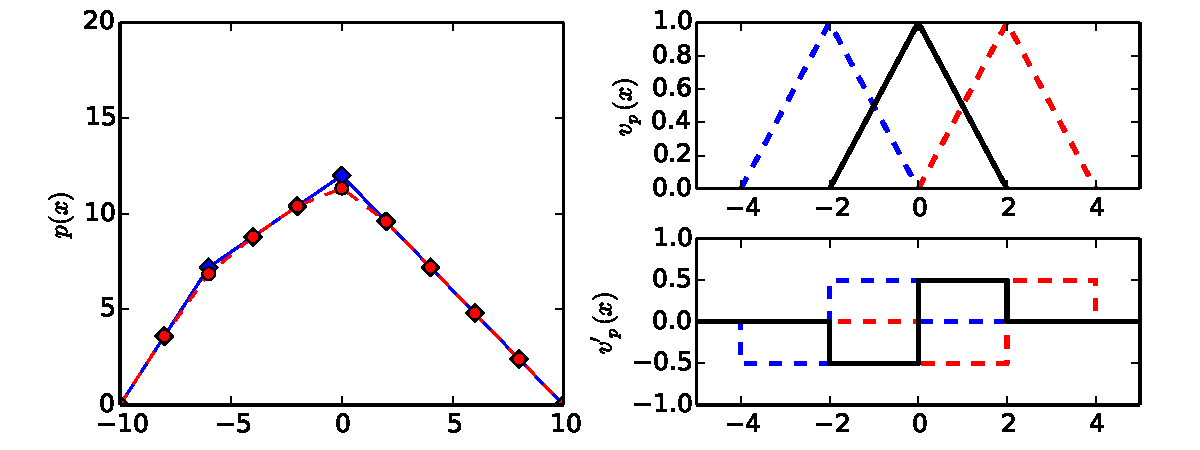
\includegraphics[width=\textwidth]{plots/fem}
	\caption{Links: Lösung des stationären Wärmeleitungsproblems mittels der FEM-Methode mit linearen Splines für $\delta$-artige (blaue Rauten) und hütchenförmige Quellen (rote Kreise). Rechts oben: die verwendeten Splines $v_p(x)$ für $p=0$ (schwarz durchgezogen), $p=-1$ (blau gestrichelt) und $p=1$ (rot gestrichelt). Rechts unten: die zugehörigen Ableitungen der Splines.}
	\label{fig:fem}
\end{figure}

Als Beispiel wollen wir die stationäre Lösung der eindimensionalen
Wärmeleitungsgleichung direkt bestimmen, also die Differentialgleichung
\begin{equation}
  D\frac{\delta^2}{\delta x^2} p(x) = -q(x)
\end{equation}
lösen, wobei $q(x)= \frac{1}{2}\,\delta\left(x+6\right) + \delta(x)$ die Wärmequellen aus dem vorherigen Beispiel sein sollen. Gesucht ist die Lösung im Interval $\Omega=[-10,10]$ mit der Randbedingung $p(-10) = p(10) = 0$. Wir approximieren die Lösung
als Summe von linearen Splines auf einem regulären Gitter der Weite $h=2$, d.\,h.\, unsere
Basisfunktionen sind (vgl. Abbildung~\ref{fig:fem}):
\begin{equation}
	v_p(x) = \begin{cases}
		x/h - p - 1 & \text{für } p - 1 \le x/h \le p \\  
		p + 1 - x/h & \text{für } p \le x/h \le p + 1 \\
		0 & \text{sonst}
		\end{cases}\quad,\, p=-4(1)4.
\end{equation}
Dies mag zunächst seltsam erscheinen, da ja die zweite Ableitung einer solchen Funktion fast überall Null ist. Die Antwort ist eine partielle Integration bei der Berechnung der linksseitigen Koeffizientenmatrix $A$, durch die die zweite Ableitung verschwindet:
\begin{equation}
  a_{pq} = \int_\Omega v''_q(x)\cdot v_P(x) dx = -\int_\Omega v'_q(x)\cdot v'_p(x) =
  	\begin{cases}
	\frac{-2}{h} & \text{für } p=q \\
	\frac{1}{h}  & \text{für } \lvert p - q \rvert = 1\\
	0 & \text{sonst.}
	\end{cases}
\end{equation}
Die Matrix $A$ ist also tridiagonal mit $-2/h$ auf der Diagonalen und $1/h$ auf den Sub- und Superdiagonalen. Dies ist bis auf einen Faktor $h$ genau die Matrix, die \eqref{eq:discrdiff} für das Finite-Differenzen-Verfahren beschreibt.

Für die rechte Seite ergibt sich durch Auswerten der beiden $\delta$-Integrale
\begin{equation}
  b_p = \int_\Omega q(x)\cdot v_p(x) dx = \begin{cases}
  \frac{1}{2} & \text{für } p = -3 \\
  1           & \text{für } p = 0 \\
  0 & \text{sonst}
  \end{cases} \quad = q(x_p),
\end{equation}
also bis auf einen Faktor $h$ ebenfalls die rechte Seite, die sich auch beim Finite-Differenzen-Verfahren ergeben würde. Daher entspricht die Lösung, wie sie Abbildung~\ref{fig:fem} zeigt, auch genau dem Langzeitlimes der FDM-Lösung aus dem letzten Kapitel.

Nehmen wir nun an, dass die rechte Seite nicht mehr $\delta$-Quellen sind, sondern zwei unserer Hutfunktionen der Breite $2h$, also $\tilde q(x)= \frac{1}{2h}\,v_{-3}(x) + \frac{1}{h}v_0(x)$. Für die FDM-Lösung macht dies keinen Unterschied, da nur die Werte an den Spitze eingehen. Für den FEM-Löser hingegen müssen wir nun $b_p$ neu bestimmen:
\begin{equation}
  b_p = \int_\Omega \tilde q(x)\cdot v_p(x) dx = \frac{1}{2h}\int_\Omega v_p(x) v_{-3}(x) + \frac{1}{h}\int_\Omega v_p(x) v_0(x) dx.
\end{equation}
Eine Hutfunktion trägt dabei nicht nur zu dem Punkt bei, an dem sie liegt, sondern auch zu den benachbarten Punkten, da
\begin{equation}
  \int_\Omega v_q(x)\cdot v_p(x) =
  	\begin{cases}
	\frac{2}{3}h & \text{für } p=q \\
	\frac{1}{6}h & \text{für } \lvert p - q \rvert = 1\\
	0 & \text{sonst,}
	\end{cases}
\end{equation}
die rechte Seite wird also mittels der Hutfunktion geglättet. In unserem Fall ergibt sich
\begin{equation}
(b_-4,\ldots,b_4) = (\frac{1}{12},\frac{1}{3},\frac{1}{12},\frac{1}{6},\frac{2}{3},\frac{1}{6}, 0, 0, 0).
\end{equation}
Die Lösung mit dieser rechten Seite ist an den beiden Quellen tatsächlich etwas \enquote{runder} als die Lösung für die $\delta$-Spitzen. Eine FDM hätte diese Feinheit nur mit deutlich feinerem Gitter reproduzieren können, da sie anders als FEM keine Annahmen über das Verhalten der Funktion zwischen den Stützstellen verarbeiten kann.

Um die Genauigkeit einer FEM weiter zu verbessern, können dort zusätzliche Gitterpunkte
eingefügt werden, wo die Funktion vermutlich stark variiert (zum Beispiel in der
Nähe der Wärmequellen in unserem Beispiel). Auch höhere Splines, zum Beispiel kubische, erhöhen die Genauigkeit, sind allerdings mehrdimensional auf allgemeinen Gitter schwer überhaupt zu definieren. Die Erzeugung solcher komplexer Gitter selber erfordert
spezielle Software, die oft nicht weniger kompliziert als der eigentliche
FEM-Löser ist. In der Ingenieurspraxis kommen daher meist sehr leistungsfähige,
kommerzielle Softwarepakete zum Einsatz. Eine freie Alternative ist das Softwarepaket
DUNE~\cite{dune,duneweb}.

\subsection{Lösung mittels Fouriertransformation --- Poisson-Gleichung}
\index{Poisson-Gleichung}
\index{Lösung partieller DGLs>mittels Fouriertransformation}

Die Poisson-Gleichung
\begin{equation}
  \label{eq:poissonreal}
  \Delta  \Phi(x) = \nabla \cdot \nabla \Phi(x)  = \frac{\rho(x)}{\epsilon}
\end{equation}
spielt auch in der Elektrostatik eine zentrale Rolle, wobei $\Phi$ in
diesem Fall das Potential, $\rho$ die Ladungsverteilung und $\epsilon$
die dielektrische Konstante ist. Im Kapitel~\ref{chap:la} wurde
bereits erläutert, dass sich diese Gleichung gut mit Hilfe von
finiten Differenzen lösen lässt, und die Wiedergabe der stationären
Lösung aus dem vorigen Abschnitt unterstreicht dies.

Wie alle lineare partiellen Differentialgleichungen mit konstanten
Koeffizienten, kann Gleichung \eqref{eq:poissonreal} unter
periodischen Randbedingungen einfach in den Fourierraum übertragen
werden, da ja $\widehat{\nabla \Phi} = i n \omega \hat \Phi$. Zweimalige
Anwendung ergibt
\begin{equation}
  \label{eq:poissonft}
  -n^2\omega^2\hat\Phi_n  = \frac{\hat\rho_n}{\epsilon}
\end{equation}
wobei $\hat\Phi_n$ und $\hat\rho_n$ die Fouriertransformierten von
$\Phi$ und $\rho$ gemäß \eqref{eq:fouriercoeff} sind. Ist $x$
mehrdimensional, wird entlang jeder Dimension nacheinander
transformiert, und $n^2$ entspricht $n\cdot n = \norm{n}^2$. Danach muss
notwendigerweise $\hat\rho_0 = 0$ gelten, das System also
ladungsneutral sein. Für die übrigen Frequenzen lässt sich die
Poissongleichung nun ganz einfach durch $\hat\Phi_n =
-\hat\rho_n/\epsilon(n\omega)^2$ lösen. Um also $\Phi(x)$ zu berechnen,
transformieren wir eine diskrete Ladungsverteilung $\rho$ mit Hilfe
der FFT in den Fourierraum, lösen dort trivial die Poissongleichung,
und transformieren $\hat\Phi$ zurück.

\lstinputlisting[style=floating,firstline=10, caption={Lösung der
  Poisson-Gleichung im Fourierraum für
  $\epsilon=1$.},label=lst:poisson]{poisson.py}%

Dieses Vorgehen spielt eine wichtige Rolle bei den sogenannten
Particle-Mesh-Ewald-Methoden zur Berechnung der Schwerkraft oder
elektrostatischer Wechselwirkungen. Diese werden in
Molekulardynamiksimulationen geladener Systeme am häufigsten
eingesetzt. Kern dieser Methoden ist, die $\delta$-Spitzen diskreter
Punktladungen durch verschmierte, normalverteilte Ladungen zu
ersetzen, deren Wechselwirkung mit Hilfe von schnellen
Fouriertransformationen wie beschrieben im Fourierraum berechnet
wird. Mit einer weiteren, kleinen Korrektur für die
Ladungsverschmierung lassen sich so die elektrostatischen
Wechselwirkungen von Millionen von Teilchen in Bruchteilen von
Sekunden auf einem Großrechner berechnen.

\begin{figure}
  \centering
  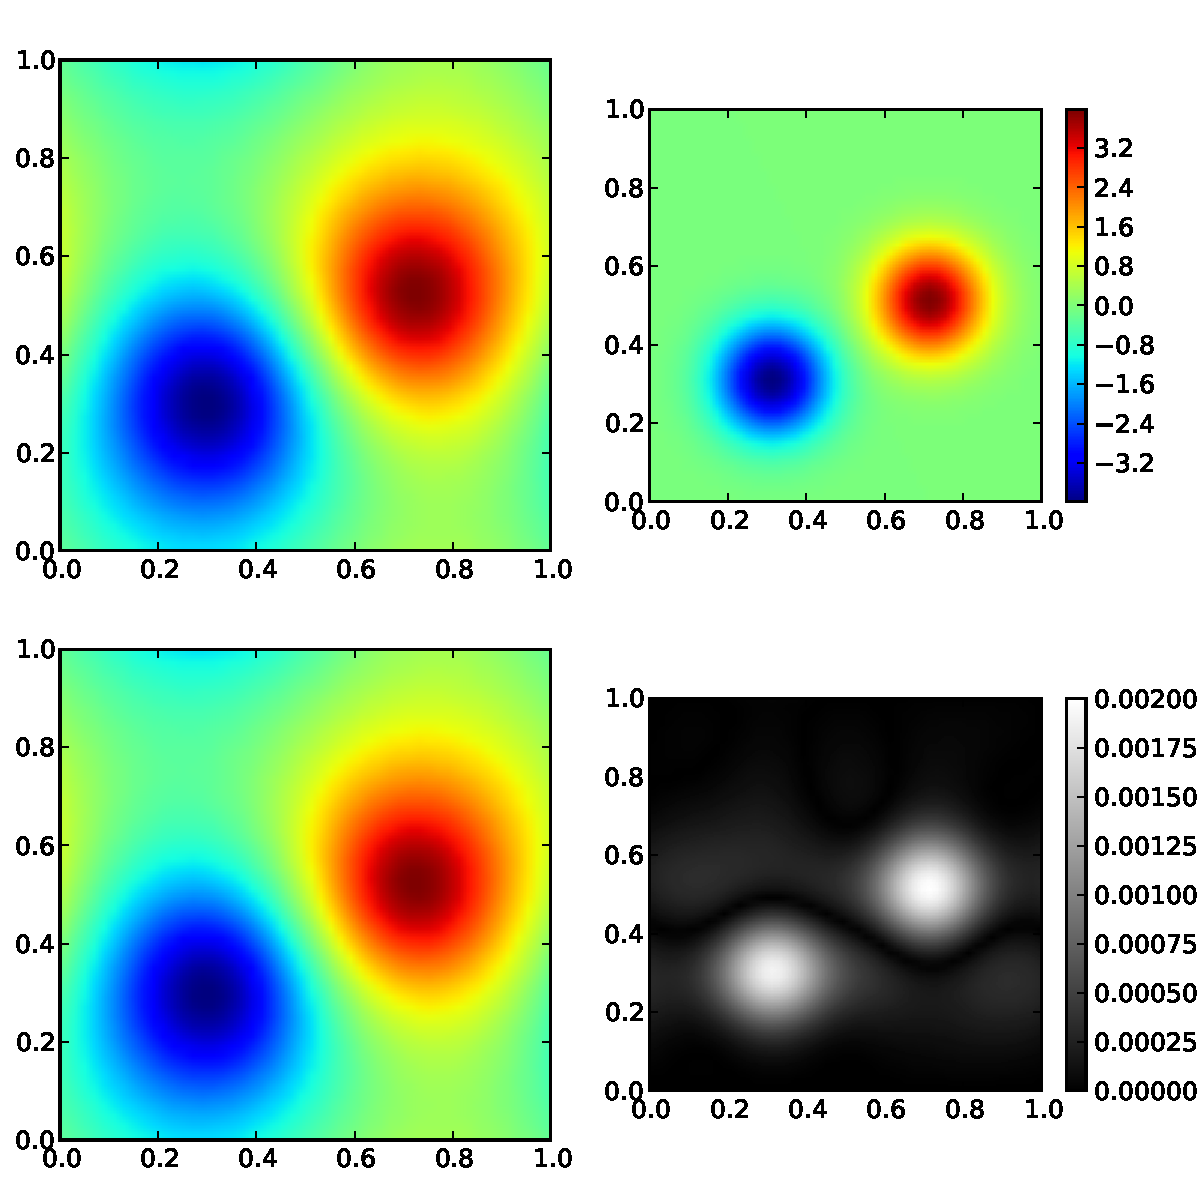
\includegraphics[width=\textwidth]{plots/poisson}
  \caption{Näherungslösung mit $50\times 50$ Gitterpunkten für die
    Poissongleichung $\Delta \Phi=\rho$ in freien
    Einheiten. Die Ladungsdichte $\rho$ ist rechts oben gezeigt
    und beinhaltet zwei normalverteilte Ladungen. Die Lösungen
    $\Phi_\text{FD}$ mit finiten Differenzen (links oben) und
    $\Phi_\text{FFT}$ im Fourierraum mittels FFT (links unten) sind
    praktisch identisch. Dies zeigt auch der relative Fehler
    $\abs{\Phi_\text{FD} - \Phi_\text{FFT}}/\abs{\Phi_\text{FFT}}$
    (rechts unten), der weniger als 2 Promille beträgt.}
  \label{fig:poisson}
\end{figure}

Codebeispiel~\ref{lst:poisson} zeigt die Lösung im Fourierraum für
eine beliebige, zweidimensionale Ladungsverteilung. In der Praxis ist
die Umsetzung des Terms $n^{-2}$ etwas komplizierter, weil bei der
diskreten Fouriertransformation die negativen Koeffizienten ja
oberhalb der positiven gespeichert sind ($\rho_{N-n}=\rho_{-n}$), und
zwar in jeder Dimension. Falls $N$ gerade ist, ist außerdem
$\rho_{N/2} = \rho_{-N/2}$, so dass man Vorsorge treffen muss, dass
dieser Wert nur einmal durch $n^2$ geteilt wird. Dies bedingt die
Fallunterscheidungen in der Implementation des Laplace-Operators.

Die Ergebnisse stimmen bis auf eine additive Konstante gut mit den
Berechnungen mittels finiter Differenzen überein, wie
Abbildung~\ref{fig:poisson} zeigt. Die Konstante rührt daher, dass die
Lösung im Fourierraum stets eine verschwindende Null-Frequenz hat,
also im Mittel Null ist. Bei der Finite-Differenzen-Lösung wird
hingegen der Wert von $\Phi$ an einer Stelle vorgegeben. Abgesehen
davon beträgt der maximale Unterschied zwischen den Lösungen weniger
als 2 Promille, und zwar genau auf den Ladungen. Ist die
Ladungsverteilung nicht glatt, so ist der Fehler größer, da die
Fouriertransformation unstetiger Funktionen ja nur langsam
konvergiert.

\subsection{Lösung der Poisson-Boltzmann-Gleichung}
\index{Poisson-Boltzmann-Gleichung}

\begin{figure}
  \centering
  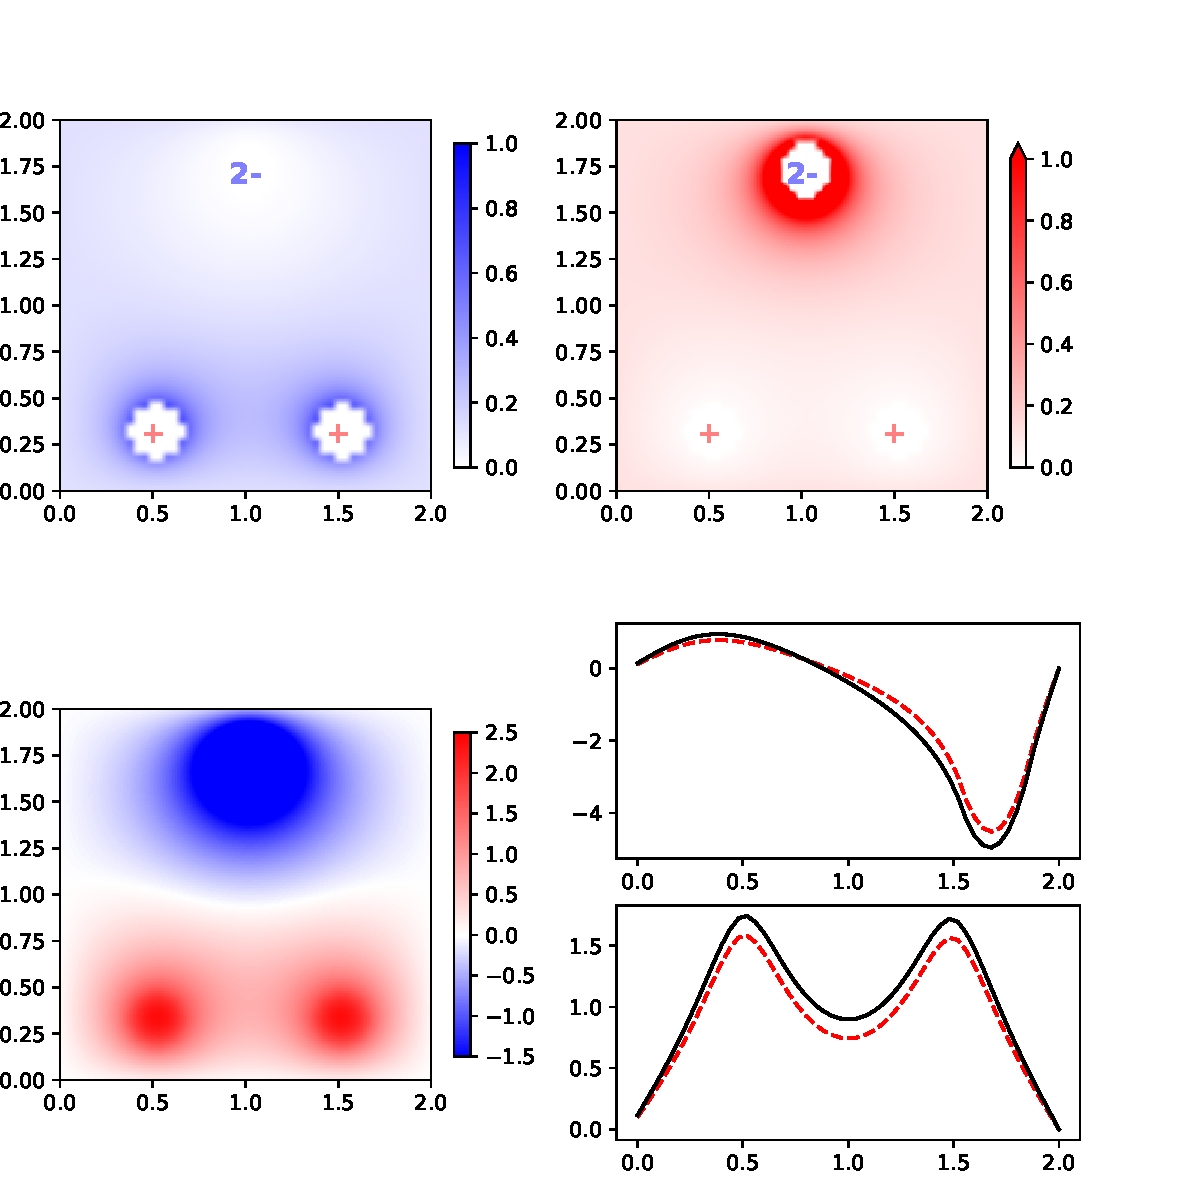
\includegraphics[width=\textwidth]{plots/pb}
  \caption{Näherungslösung der
    Poisson-Boltzmann-Gleichung~\eqref{eq:pb} mittels iterativer
    Lösung des diskretisierten Gleichungssystems. Die Ladungsdichte
    konvergiert innerhalb von zwanzig Schritten zu einer Genauigkeit
    von $10^{-2}$. Links oben ist die resultierende Verteilung der
    negativen Ionen gezeigt, rechts oben der positiven Ionen. Da die
    Ionen in die Bereiche der fixen Ladungen nicht eindringen können,
    ist dort die Ladungsdichte 0. Der ausgefranste Rand dieser
    Bereiche ist eine Folge der groben Diskretisierung. Unten links
    ist das resultierende Potential dargestellt, rechts unten die
    Potentialverläufe des Poisson-Boltzmann-Potentials (rot
    gestrichelt) und des reinen elektrostatischen Potentials
    (durchgezogen). Der obere der beiden Graphen zeigt
    $\psi(1,y)$, der untere $\psi(x, 1/2)$.}
  \label{fig:pb}
\end{figure}

Als letztes Beispiel wollen wir eine wichtige Erweiterung der
Poisson-Gleichung lösen, die Poisson-Boltzmann-Gleichung. Für die
Herleitung dieser Gleichung nehmen wir an, dass neben der fixen
Ladungsverteilung $\rho_\text{fix}(x)$ noch ein gelöstes Salz aus
einwertigen, punktförmigen Ionen im System ist. Das Salz kann sich
frei in einem Bereich $\Omega$ bewegen. Dieser wird durch die
charakteristische Funktion $\chi(x)$ charakterisiert, die für
$x\in\Omega$ den Wert 1 annimmt, und sonst 0 ist. Die räumliche
Verteilung dieser Ionen im Gleichgewicht ist durch die
Boltzmannverteilung gegeben, also proportional zu
$e^{-q\beta\Phi(x)}$, wobei $\beta=k_BT$ mit der Boltzmann-Konstanten
$k_B$ und Temperatur $T$. $q$ ist dabei die Ladung der Ionen, hier
eine negative oder positive Elementarladung. Die Einschränkung auf
monovalente Ionen hat einen guten Grund: für mehrwertige Salze kann
man zeigen, dass die Poisson-Boltzmann-Gleichung keine gute Näherung
ist.

Das Potential erscheint also auch in der Verteilung der Ionen, so dass
wir eine nichtlineare Differentialgleichung erhalten:
\begin{align}
  \epsilon\Delta \Phi(x)  &=
  -\rho_\text{fix} - c_\infty \left(q_e\underbrace{e^{-\beta
        q_e\Phi(x)}}_\text{positive Ionen} -q_e\underbrace{e^{\beta
        q_e\Phi(x)}}_\text{negative Ionen}\right)\chi(x)\nonumber\\
  &=
  -\rho_\text{fix} - 2c_\infty\sinh[-\beta q\Phi(x)]\chi(x).
\end{align}
$c_\infty$ ist dabei die Konzentration der Ionen weit von allen
Ladungen entfernt, also dort, wo $\Phi=0$. $q_e$ bezeichnet hier die
Elementarladung, um einer Verwechslung mit der Eulerschen Konstanten
vorzubeugen. Durch die Multiplikation mit $\chi(x)$ befinden sich die
Ionen nur im zulässigen Bereich, unabhängig vom Potential.

Die Gleichung lässt sich etwas einfacher darstellen, wenn man die
sogenannte Bjerrumlänge
\begin{equation}
  l_B = \frac{q_e^2}{4\pi\epsilon k_BT}
\end{equation}
einführt, und die dimensionslose Funktion $\psi=\beta q_e\Phi$ sucht,
für die dann
\begin{equation}
  \label{eq:pb}
  \frac{1}{4\pi l_B}\Delta \psi(x) =
  -q_\text{fix} - 2c_\infty\sinh[-\psi(x)]\chi(x)
\end{equation}
gilt, wobei $q_\text{fix} = \rho_\text{fix}/q_e$ die feste
Ladungsverteilung in Elementarladungen angibt. $l_B$ ist eine Konstante,
die das umgebende Medium beschreibt. Üblicherweise ist dieses Wasser,
für dass die Bjerrumlänge $0,7$nm beträgt.

Die Poisson-Boltzmann-Gleichung wird zum Beispiel benutzt, um die
Ladungsverteilung um makroskopische Ionen wie kolloidale Teilchen zu
modellieren. Dadurch muss die sehr große Menge an Salzionen nicht
explizit modelliert werden, was die Zahl der Teilchen in Grenzen
hält. In der Biophysik wird die Poisson-Boltzmann-Verteilung auch
gerne zur Visualisierung der Ladungsverteilung von Proteinen benutzt.

Ist das Potential relativ flach, lässt sich die
Poisson-Boltzmann-Gleichung mittels $\sinh(\psi)\approx \psi$
linearisieren und in manchen Geometrien analytisch lösen. Die volle,
nichtlineare Poisson-Boltzmann-Gleichung muss aber numerisch
gelöst werden. Dazu diskretisieren wir $\psi$ wieder äquidistant in
beiden Raumrichtungen, und ersetzen den Laplace-Operator durch eine
finite Differenz. Im Prinzip könnten wir nun das Gleichungssystem mit
Hilfe des Newtonverfahrens lösen, einfach ist aber die iterative
Lösung mittels
\begin{equation}
  \psi^{(n+1)}(x)  = -\Delta^{-1}\left\{
    4\pi l_Bq_\text{fix} + 2c_\infty\sinh[-\psi^{(n)}(x)]\chi(x)\right\}.
\end{equation}
Dabei wird natürlich nicht die Inverse des diskretisierten
Laplace-Operators berechnet, sondern das Gleichungssystem gelöst. Da
dies in jeder Iteration geschehen muss, berechnet man sinnvollerweise
eine LR-Berechnung voraus, und benutzt in den Iterationen nur eine
schnelle Vorwärts- und Rückwärtssubstitution.

Listing~\ref{lst:pb} zeigt eine Implementation dieses iterativen
Poisson-Boltzmann-Lösers, Abbildung~\ref{fig:pb} die Lösung für ein
sehr einfaches System aus drei homogenen Ladungsscheiben in zwei
Dimensionen (bzw.\ drei geladenen, unendlich langen Stäben). Die
Scheibe oben hat eine Gesamtladung von 2 Elementarladungen, die beiden
unteren jeweils eine Elementarladung. Das Salz ist $0,2$-molar, die
Längeneinheit entspricht einen Nanometer, die Bjerrumlänge ist für
Wasser gewählt, also $0,7$nm. Wie erwartet finden sich die negativen
Ionen bevorzugt in der Umgebung der beiden positiven Kugeln unten, die
positiven Ionen hingegen bei der größeren, negativen Kugel oben. In
diesem Beispiel konvergiert die Iteration in etwa zwanzig Schritten
auf $10^{-2}$ Genauigkeit in der Ladungsverteilung.

Rechts unten zeigt Abbildung~\ref{fig:pb} schließlich zwei Schnitte
durch das elektrostatische Potential. Dies wurde einmal nur für die
fixen Ladungen berechnet, und einmal für die
Poisson-Boltzmann-Lösung. Deutlich sichtbar ist, dass diese flacher
ist als die das reine elektrostatische Potential. Dies ist einfach zu
verstehen, da die Ionen sich ja bevorzugt um die entgegengesetzt
geladenen Bereiche anlagern, und diese dadurch gegeneinander
abschirmen.

Obwohl im Beispiel die Auswirkungen auf das Potential scheinbar nur
gering sind, ist das Poisson-Boltzmann-Potential sehr verschieden vom
klassischen elektrostatischen Potential. Um dies zu zeigen, betrachten
wir eine einzelne Punktladung. Dann ist das Potential $\psi$
radialsymmetrisch und erfüllt fern von der Ladung
\begin{equation}
  \Delta \psi(r) =\frac{\partial^2}{\partial r^2} \psi(r)
  +\frac{2}{r}\frac{\partial}{\partial r} \psi(r) =
  -8\pi l_B c_\infty\sinh[-\psi(r)] \approx 8\pi l_B c_\infty\psi(r),
\end{equation}
wobei wir für die letzte Näherung annehmen müssen, dass $\psi$ bereits
hinreichend stark abgefallen ist. Diese Gleichung, die sogenannte
Debye-Hückel-Näherung, ist schließlich analytisch lösbar und hat die
Lösung $\psi(r) = e^{-\kappa r}/r$
mit $\kappa = \sqrt{8\pi l_B c_\infty}$, wie man sich leicht
überzeugt. Das Coulomb-Potential ist also exponentiell gedämpft, wobei
die charakteristische Länge der Dämpfung $\kappa^{-1}$ ist. Für eine
0,1-molare Salzlösung (was in etwa dem Zellplasma entspricht) beträgt
sie nur etwa $1$nm, \dh es gibt praktisch keine elektrostatischen
Wechselwirkungen über Distanzen größer als ein Nanometer.

\lstinputlisting[style=floating,firstline=10, caption={Python-Code zur
  Poisson-Boltzmann-Gleichung. Die Lösung wird räumlich mittels
  finiter Differenzen erster Ordnung diskretisiert und anschließend
  durch Bestimmen des Potentials aus der aktuellen Ladungsdichte
  iterativ bestimmt.},label=lst:pb]{pb.py}%

%%% Local Variables: 
%%% mode: latex
%%% TeX-master: "padc.tex"
%%% TeX-PDF-mode: t
%%% End: 
